% Conclusion chapter timeline — Chapter 7
% Three-phase forward-looking judgment timeline: Prototype Verification → Limited Deployment → Conditional Expansion
% Explicitly designated as a forward-looking judgment timeline, not a historical event review
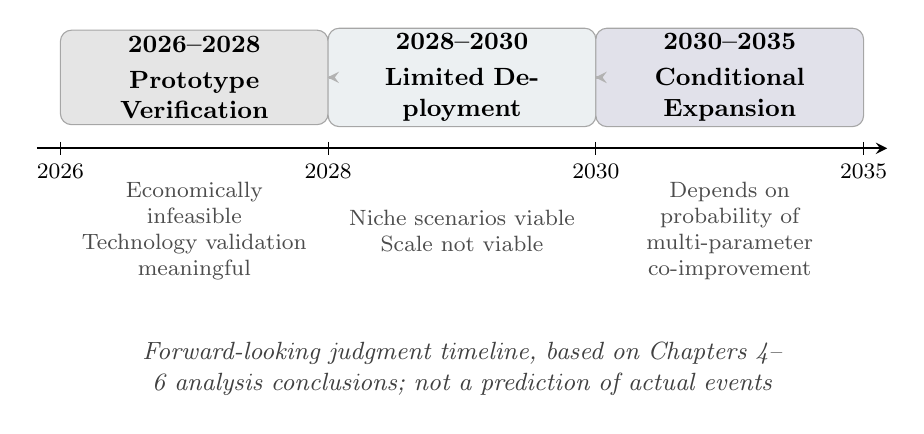
\begin{tikzpicture}[
  phase/.style={rectangle, draw=gray!70, rounded corners, minimum width=3.4cm, text width=3.2cm,
                minimum height=1.2cm, align=center, font=\small, inner sep=2pt},
  judge/.style={text width=3.0cm, align=center, font=\footnotesize, text=black!70},
  arrow/.style={thick, draw=gray!60, ->, >=stealth},
  note/.style={text width=0.85\textwidth, font=\small\itshape, text=gray!50!black,
               align=center, inner sep=4pt}
]
  % ===== Bottom time axis =====
  \draw[thick, ->, >=stealth] (-0.3,0) -- (10.5,0);

  % Time ticks — aligned with phase boundaries
  \foreach \x/\l in {0/2026, 3.4/2028, 6.8/2030, 10.2/2035}
    \draw (\x,0.08) -- (\x,-0.08) node[below, font=\footnotesize] {\l};

  % ===== Phase 1: 2026--2028 Prototype Verification =====
  \node[phase, fill=gray!20] (p1) at (1.7,0.9) {\textbf{2026--2028}\\[2pt]\textbf{Prototype Verification}};
  \node[judge] at (1.7,-1.05) {Economically infeasible\\Technology validation\\meaningful};

  % ===== Phase 2: 2028--2030 Limited Deployment =====
  \node[phase, fill=cyan!18!gray!14] (p2) at (5.1,0.9) {\textbf{2028--2030}\\[2pt]\textbf{Limited Deployment}};
  \node[judge] at (5.1,-1.05) {Niche scenarios viable\\Scale not viable};

  % ===== Phase 3: 2030--2035 Conditional Expansion =====
  \node[phase, fill=blue!16!gray!20] (p3) at (8.5,0.9) {\textbf{2030--2035}\\[2pt]\textbf{Conditional Expansion}};
  \node[judge] at (8.5,-1.05) {Depends on probability of\\multi-parameter\\co-improvement};

  % ===== Inter-phase evolution arrows =====
  \draw[arrow] (p1.east) -- (p2.west);
  \draw[arrow] (p2.east) -- (p3.west);

  % ===== Bottom note =====
  \node[note] at (5.1,-2.8) {Forward-looking judgment timeline, based on Chapters~4--6 analysis conclusions; not a prediction of actual events};
\end{tikzpicture}
